
\chapter{Exploration 5: exploring what time scrubbing mechanisms XIMPEL needs}
% Question: what are the technical requirements and difficulties for creating time scrubbing in XIMPEL?

During my talks with Hugo Huurdeman we both came independently to the conclusion what XIMPEL should have a time scrubbing feature that is related to all media types but especially video. I talked about how to possibly implement this. Then, as I went on to implement it, I gradually realized that a time scrubbing feature for multiple parallel playing media is not straightforward at all. For this reason, I staved off development and thought about the different possible conceptual implementations of this. Time scrubbing in multiple parallel playing media is not the same compared to time scrubbing for one video. Different conceptual implementations will lead to very different behavioral outcomes when a user starts to use the time scrubbing feature. Since few people thought about this before, I will attempt to outline different time scrubbing scenarios. Unfortunately, no time scrubbing mechanism is implemented since there are too many design questions. The presentation and illustration of these questions is the result of this exploration.


%There are 3 problems with time scrubbing:
%Normal time scrubbing with parallel media
%Time scrubbing and overlays
%Time scrubbing and subjects

\section{Time scrubbing with videos}
In normal videos time scrubbing is straightforward. There is a slider. With this slider the user is able to control at what time playback starts or skips to (see figure \ref{fig:normal_time_scrubbing}). From a user experience standpoint the benefits are: being able to skim videos by time scrubbing through it, skipping unnecessary parts by showing small relevant segments and replaying a small segment after having not fully seen it due to a lack of focus, for example.

The straightforwardness comes from the fact that videos are linear media. Time scrubbing allows for random access of linear media. Furthermore, videos are only one instantiation of media. Multiple videos playing at the same time would be multiple instantiations of media. Contrast that with media played in XIMPEL which could be: non-linear and have multiple instantiations of different forms of media such as one text block, two images, three audio tracks, four videos and five custom defined animations.

\begin{figure}
\centering
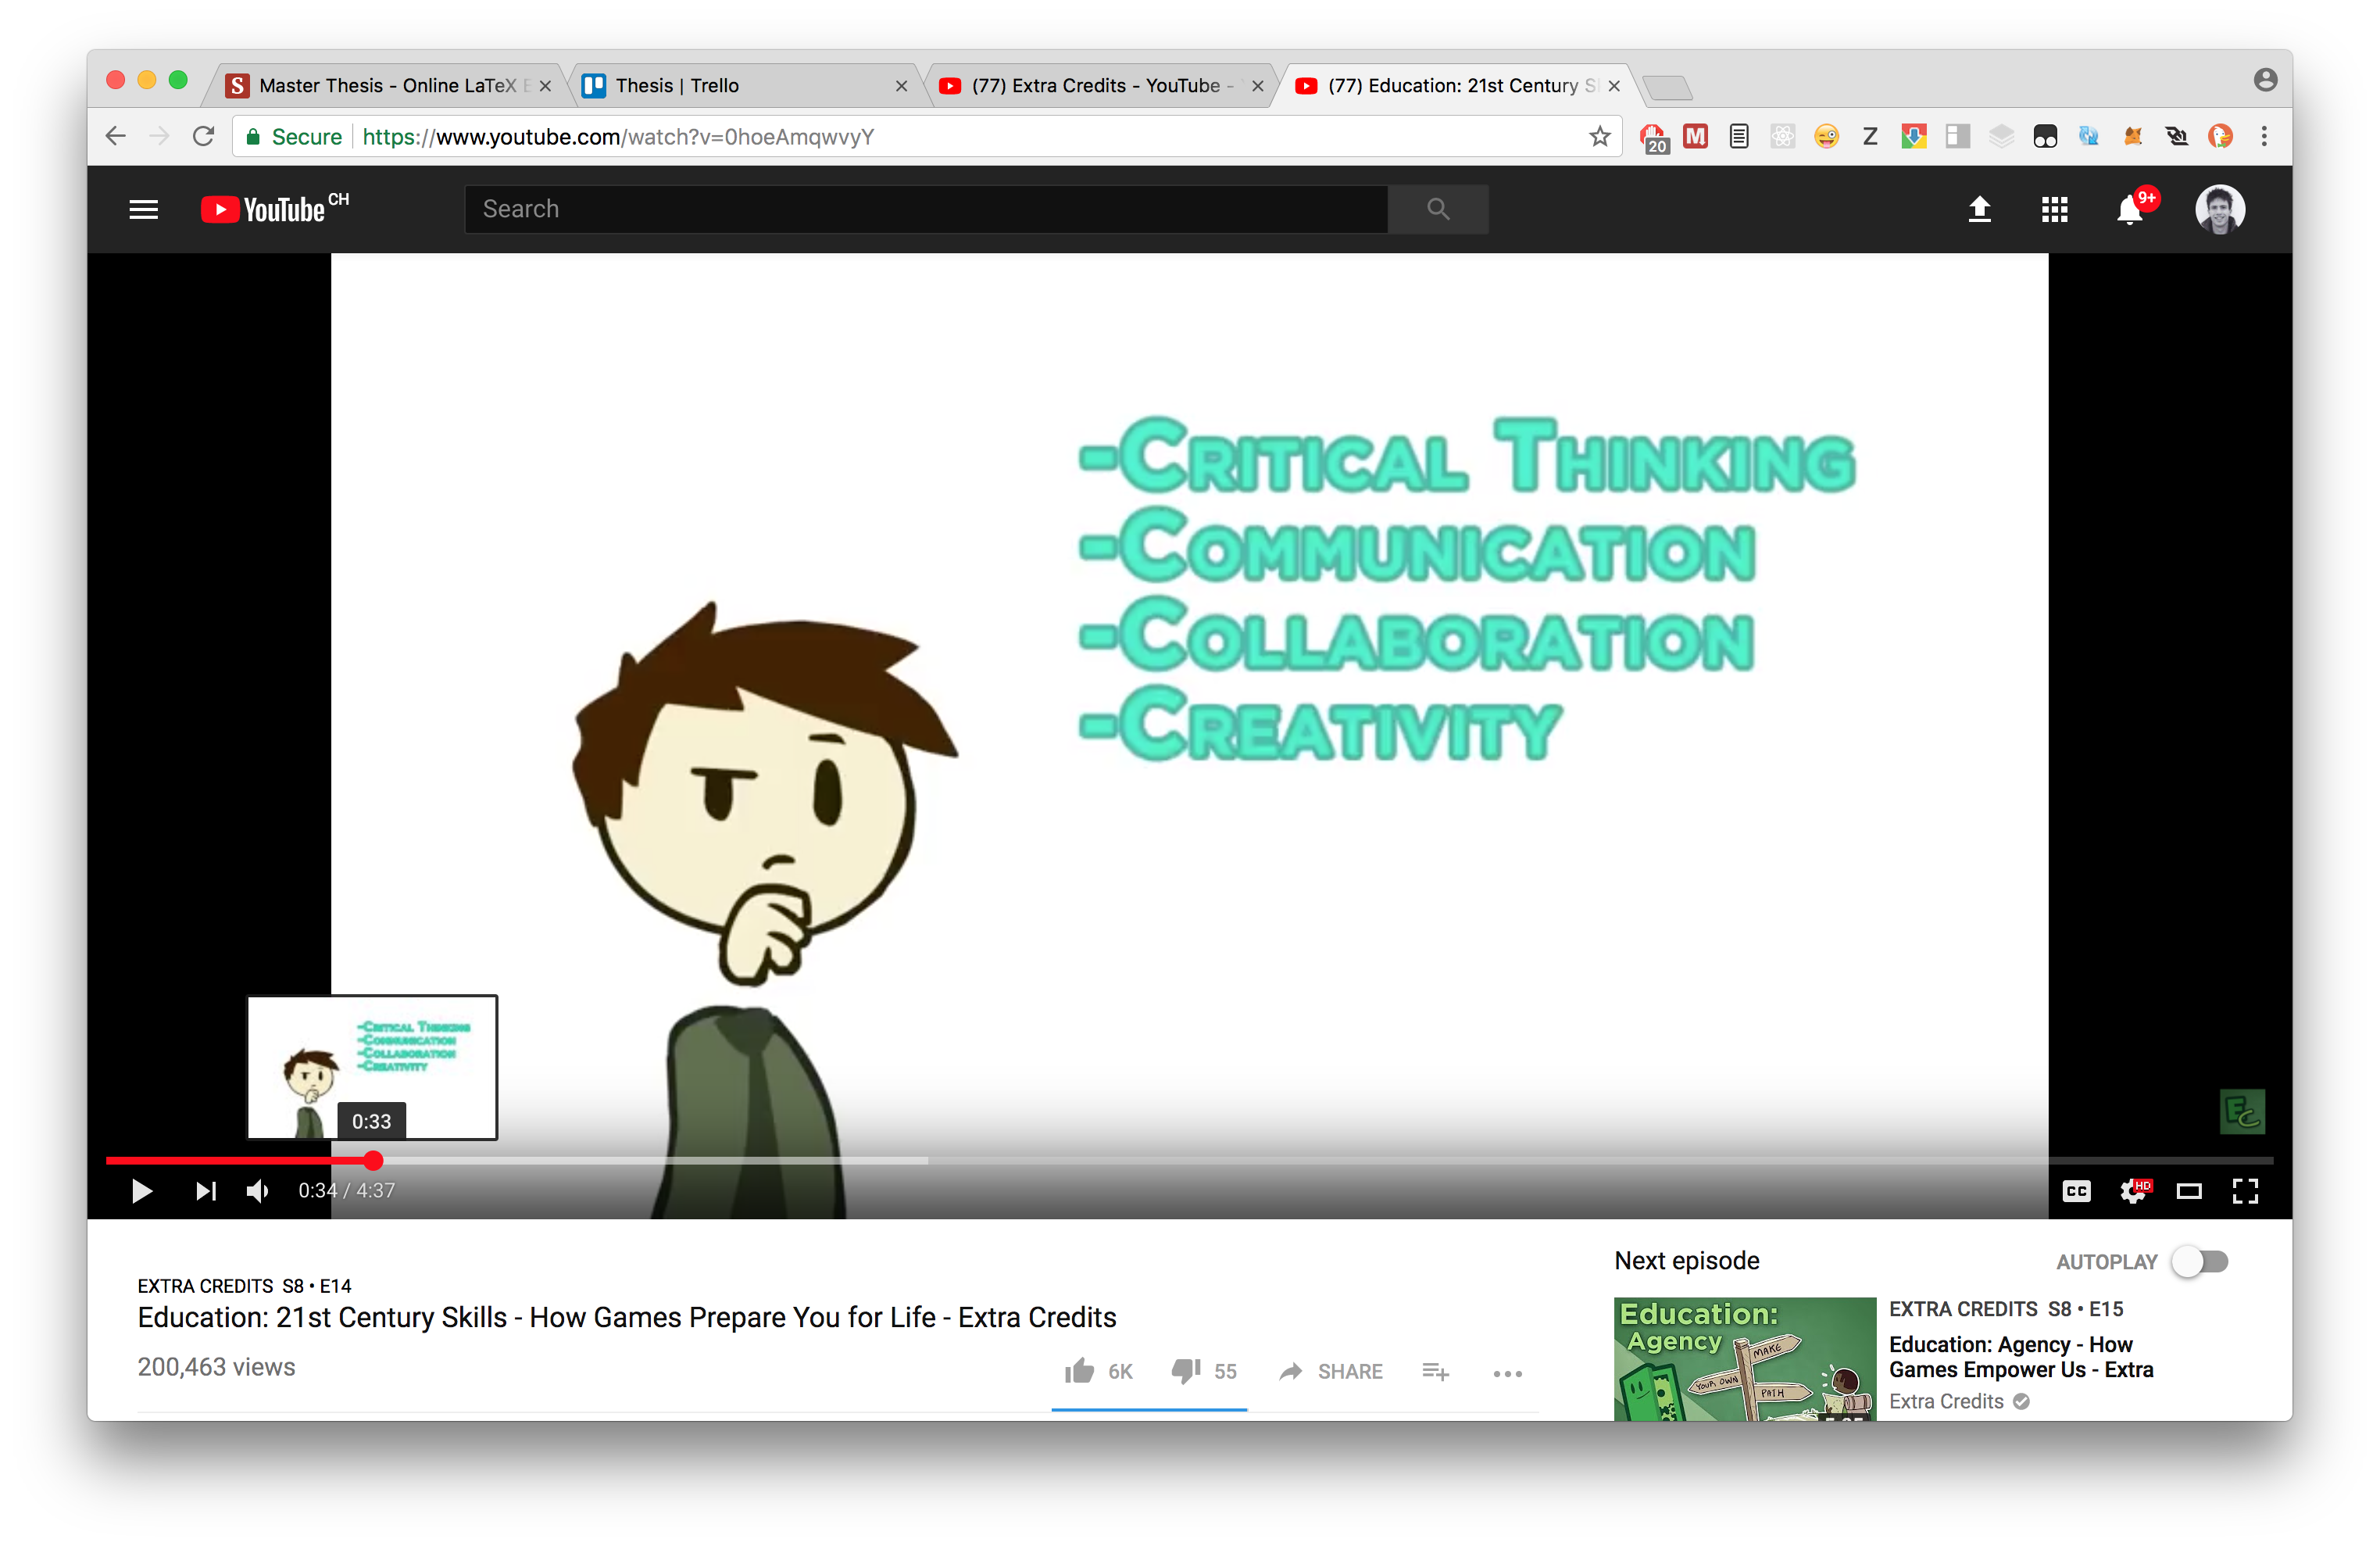
\includegraphics[width=1.35\textwidth, center]{time_scrubbing_mechanism.png} % quotation marks make sure file name does not display
\caption{An example of time scrubbing with a YouTube video. The red line could be dragged by the mouse to earlier or later times and resume playback there. The video itself is taken from a show called Extra Creditz, which talks about how game-design affects our lives for the better.}
\label{fig:normal_time_scrubbing}
\end{figure}

\section{Related work}
Before we start getting into the wonderland that is time scrubbing let us first look at related work in order to have some background knowledge. Some researchers also decided to present their work on YouTube which is arguably gives a much more intuitive introduction. The in-text citations of these papers are made \textbf{bold} (e.g. \textbf{[1337]}). When you, dear reader, look at the bibliography a YouTube URL will be there for you, so you can watch a demonstration of their work. Since we are going to look at time scrubbing systems it may be useful to first see systems in action rather than read academic articles.

Previous research on time scrubbing and related video browsing methods has mostly -- if not only -- been done for linear videos. In my own literature research I found that the biggest trend in time scrubbing research has been manipulating objects in video \cite{nguyen2013, shah2013, goldman2008, dragicevic2008, kimber2007}. The idea is that by manipulating an object within the video, a user is able to scrub along. 

Thumbnail like strategies are another way of doing this. For example, one study presented an interface in which a user sees still images of the video in a grid on their smartphone. When a user taps on one of these images, another set of still images are shown that are closer in time around the first tapped still image \cite{hi_story2012}. Another example is a study that used still images in a tree like fashion. The deeper levels presented still images for more fine-grained time scrubbing control whereas the levels closer to the root node were more coarse \cite{videotree2010}.

Then, there is a line of research that improves the experience of time scrubbing in some sort of fashion. For example, by implementing multiple time scrub bars \cite{multipletimeline1999}, altering the time scrubbing experience \cite{dynamictime2010}, by having automatic labels above or below the time scrub bar \cite{automaticsection2015} or manual ones\footnote{The custom-made video player of the Harvard course CS50: Introduction to Computer Science does this.} or by altering fast-forwarding functionality \cite{fastforward2009}.

Specifically for our interest, time scrubbing or related video browsing techniques have been developed purely for education and MOOCs. In one study, researchers improved the time scrub bar by looking at user statistics. Sections on the scrub bar where it has been stopped at or played at most were highlighted and when a user went over it with the mouse cursor it felt a bit resistant to continue to a non-highlighted part. It furthermore offers a search bar to search text in the transcript, which is mapped to the time it was said in the video. Finally, the most watched parts of the lecture have been automatically summarized. \cite{kim2014}. In another study, researchers created a complete system meant for YouTube educational videos. They created a word cloud in which they utilized the x-axis (temporal ordering in the video), y-axis (temporal spread), font-size (prominence) and font-color (level of acoustic stress). They furthermore created a second word cloud that summarizes a part of the video. A third feature they have are video slides that show points of interest for the next and previous slides, they also have a time scrub bar, which indicates on some points the auditory stress on certain concepts \cite{yadav2015}.

%Review
More information on this topic can be found in the literature review of Schoeffmann, Hudelist and Huber \cite{schoeffmann2015}. The previous information has been found by conducting my own literature search. The literature survey of Schoeffmann et al. is more comprehensive. However, the work of the following authors is not included in the review \cite{shah2013, goldman2008, dragicevic2008, kimber2007, multipletimeline1999, automaticsection2015, fastforward2009, kim2014, yadav2015}. This means that some work of 2013 and 2014 that I cited is not included and all works that I cited before 2009 and the year 2015 are not included. 


%Conclusions
Most conclusions of the reviewers are relevant for our purposes with XIMPEL. The reviewers found that many of the video browsing tools ``try to follow metaphors from real life, such as film strips, multiple parallel, displays and simulated tape recorders.'' Also, ``many interfaces make use of the third dimension.'' Most important of all, ``it is also observable that many tools try to make navigation in videos more convenient by using concepts like sliders with rubber band effects, direct manipulation of objects and synchronized display of thumbnails.'' \cite{schoeffmann2015} It is important to note that these are all conclusions based on what researchers and developers create. The conclusions cannot necessarily be drawn for the user or user experience. As of now, it is still not known to what extent users are waiting for these type of improvements. 

% Biggest critique of the review is no user evaluation
The reviewers formulated their biggest critique related to it: many studies did not perform a user evaluation. This means that a lot of studies have been peer reviewed and published on the idea of: having a justification based on an intuition, looking for related work, designing an own system and -- in most but not all cases -- presenting a prototype. 

%theory of users: scrub bar and watching video
Moreover, my own observation from the literature review is that very few theories and conceptual ideas about user behavior have been formed. There is, however, one study that did look at user behavior and attempted to infer a simple model out of that behavior. The researchers noticed that users mainly use the time scrub bar or simply watch the video from beginning and forward skip in time by a little bit, mostly using the mouse, and possibly restart the video to find what they need. What they did not do was make an educated guess and immediately jump to a specific point in time \cite{cobarzan2014}. 

% Hypervideo 360º
Unrelated, but worth mentioning is that one study in the literature review called 360 degree viewable video by the term \textit{hypervideo} \cite{neng2010}. This may indicate that previous research on hypervideo between 1990 and 2009 is a bit forgotton and now everything that extends the idea of video could potentially be called hypervideo.

\section{Within subject time scrubbing in XIMPEL}
Without the parallel media player, time scrubbing in XIMPEL is a straightforward concept. The way one would scrub with YouTube can be copied and pasted to any media type in XIMPEL -- including text, images and audio. 



% A XIMPEL application in purely sequential mode can be modeled as a directed graph of subjects as $G = (V, E)$ for which $V$ is the collection of subjects and $E$ denotes the direction of a transition from one subject to the next. This graph can be a tree or a graph with cycles, jumping from one subject to the next and back to the previous subject (completing the cycle). 

% Do you have multiple YouTube videos that you can manipulate individually? Or should it be at the level of a subject?

\subsection{Time scrubbing: the difficulties introduced by the parallel player}
%scrubbing within a subject
However, combining time scrubbing with the parallel player makes it more complicated. Now, a subject has control over multiple media types playing at the same time. The first question that make this question complicated is: (idea 1) should the user be able to control time scrub bars of individual media items? (idea 2) Or should the user be able to manipulate a global time scrub bar that will slide all the media items at once? The next two figures show the distinction visually. The visual example is only with videos. It is left as an exercise to the reader to imagine this with mixed media types (see figure \ref{images:local_scrub_bars} and \ref{images:global_scrub_bar_only}). 

\begin{figure}
\centering
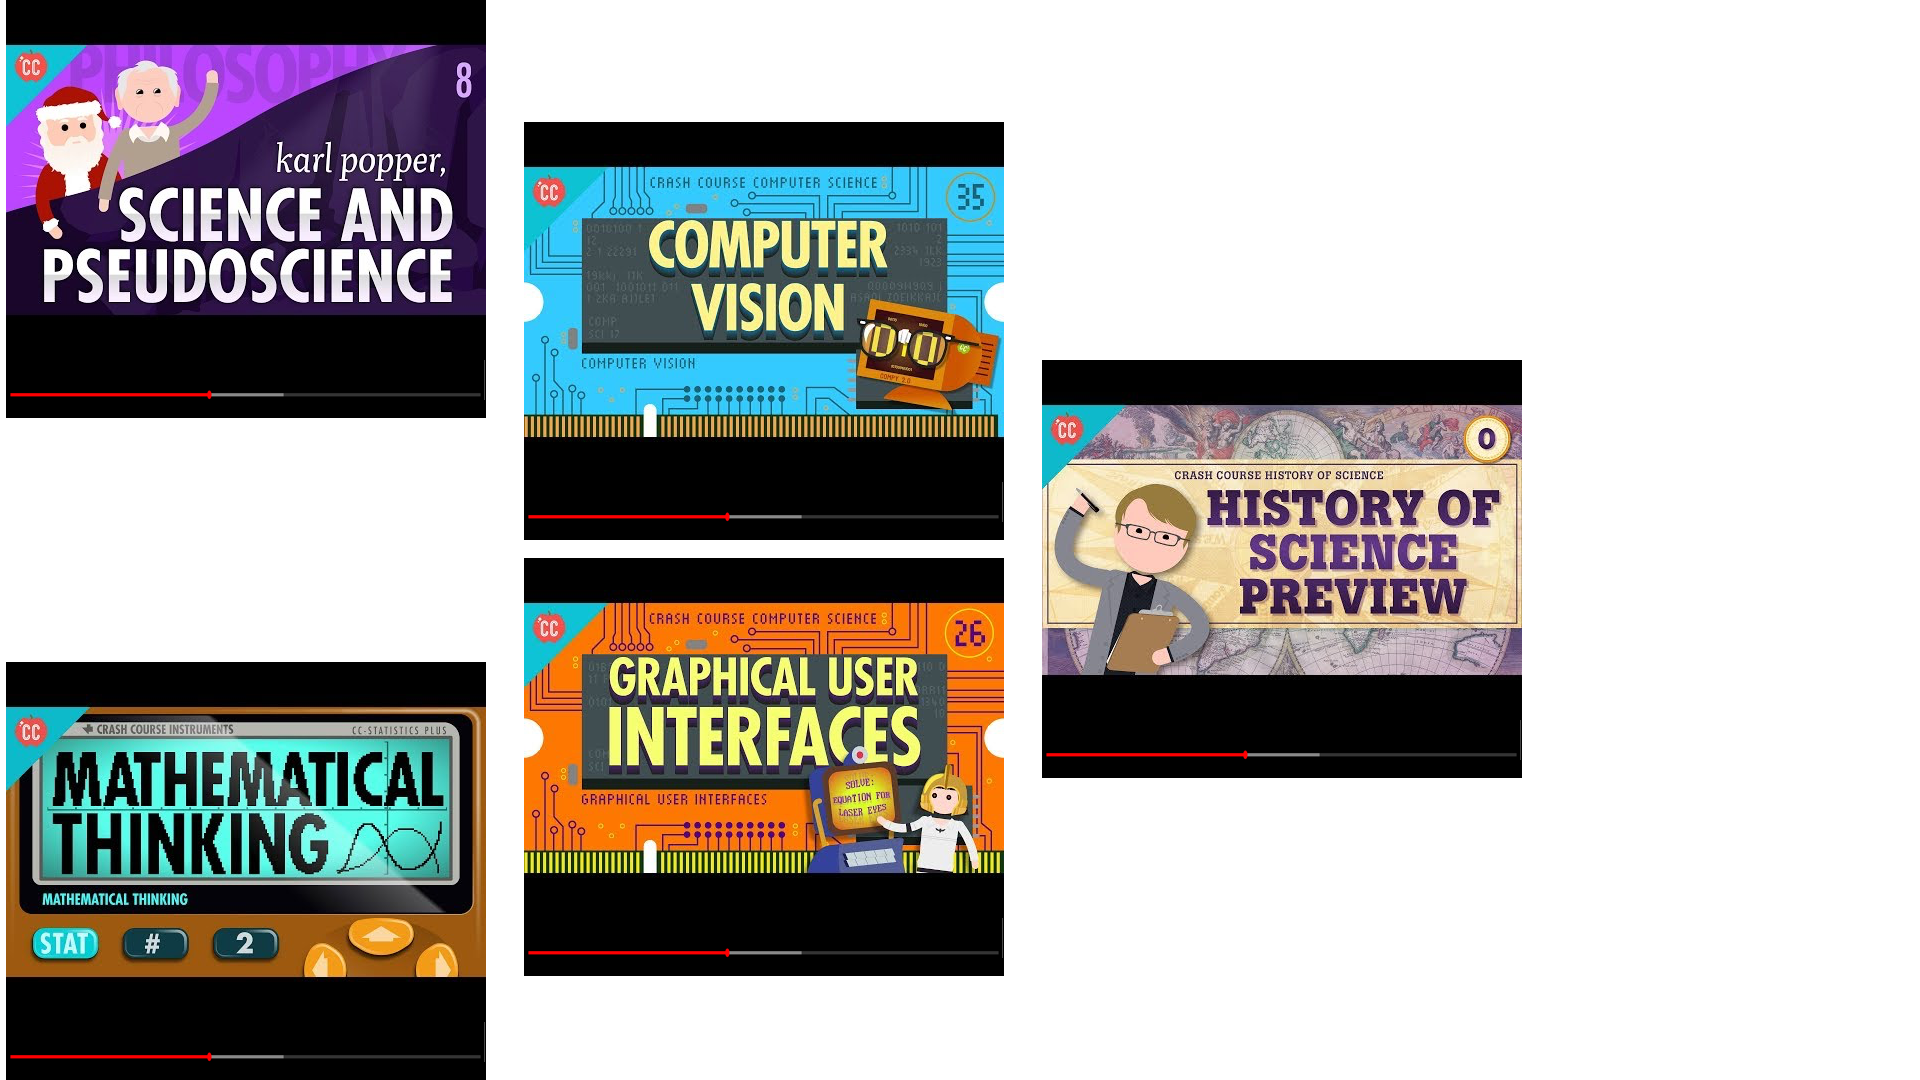
\includegraphics[width=1.35\textwidth, center]{images/local_scrub_bars.png} % quotation marks make sure file name does not display
\caption{An example of how local scrub bars look like. They are completely independent of each other, and it is unknown to each scrub bar that there are other scrub bars and at what time they are resuming playback. Image credit: thumbnails from the educational show Crash Course (on YouTube).}
\label{images:local_scrub_bars}
\end{figure}

\begin{figure}
\centering
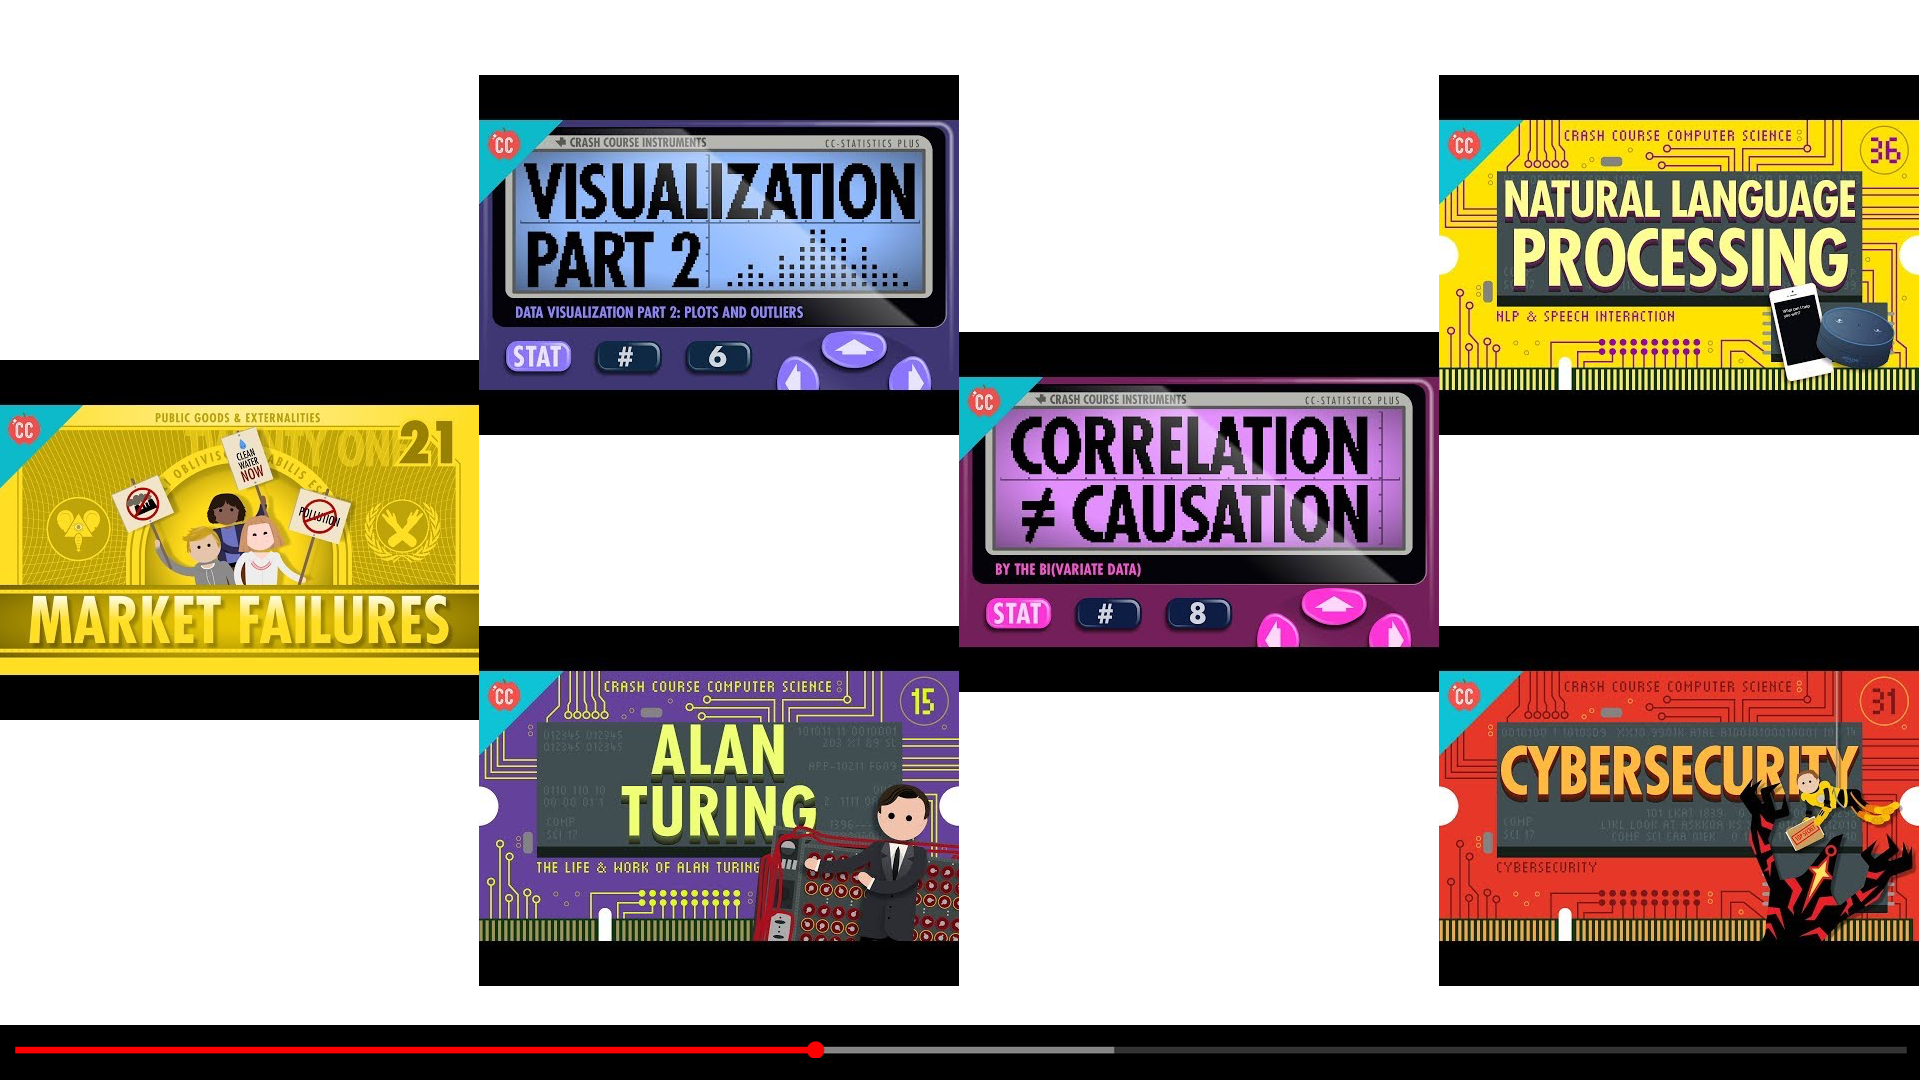
\includegraphics[width=1.35\textwidth, center]{images/global_scrub_bar_only.png} % quotation marks make sure file name does not display
\caption{An example of how a global scrub bar looks like. One scrub bar manipulates the time for all media items in the presentation. Image credit: thumbnails from the educational show Crash Course (on YouTube).}
\label{images:global_scrub_bar_only}
\end{figure}

Manipulating the individual time scrub bars is still fairly straightforward (idea 1 and figure \ref{images:local_scrub_bars}), since the interface does not change. The time scrub bar interface simply displayed more often in the XIMPEL application. The complicatedness, increases when one tries to answer the second question (idea 2 and figure \ref{images:global_scrub_bar_only}). It could be argued to choose for either ideas (1, the local multiple time scrub bars or 2, the global time scrub bar), both ideas need to have a conceptual realization.

\begin{figure}
\centering
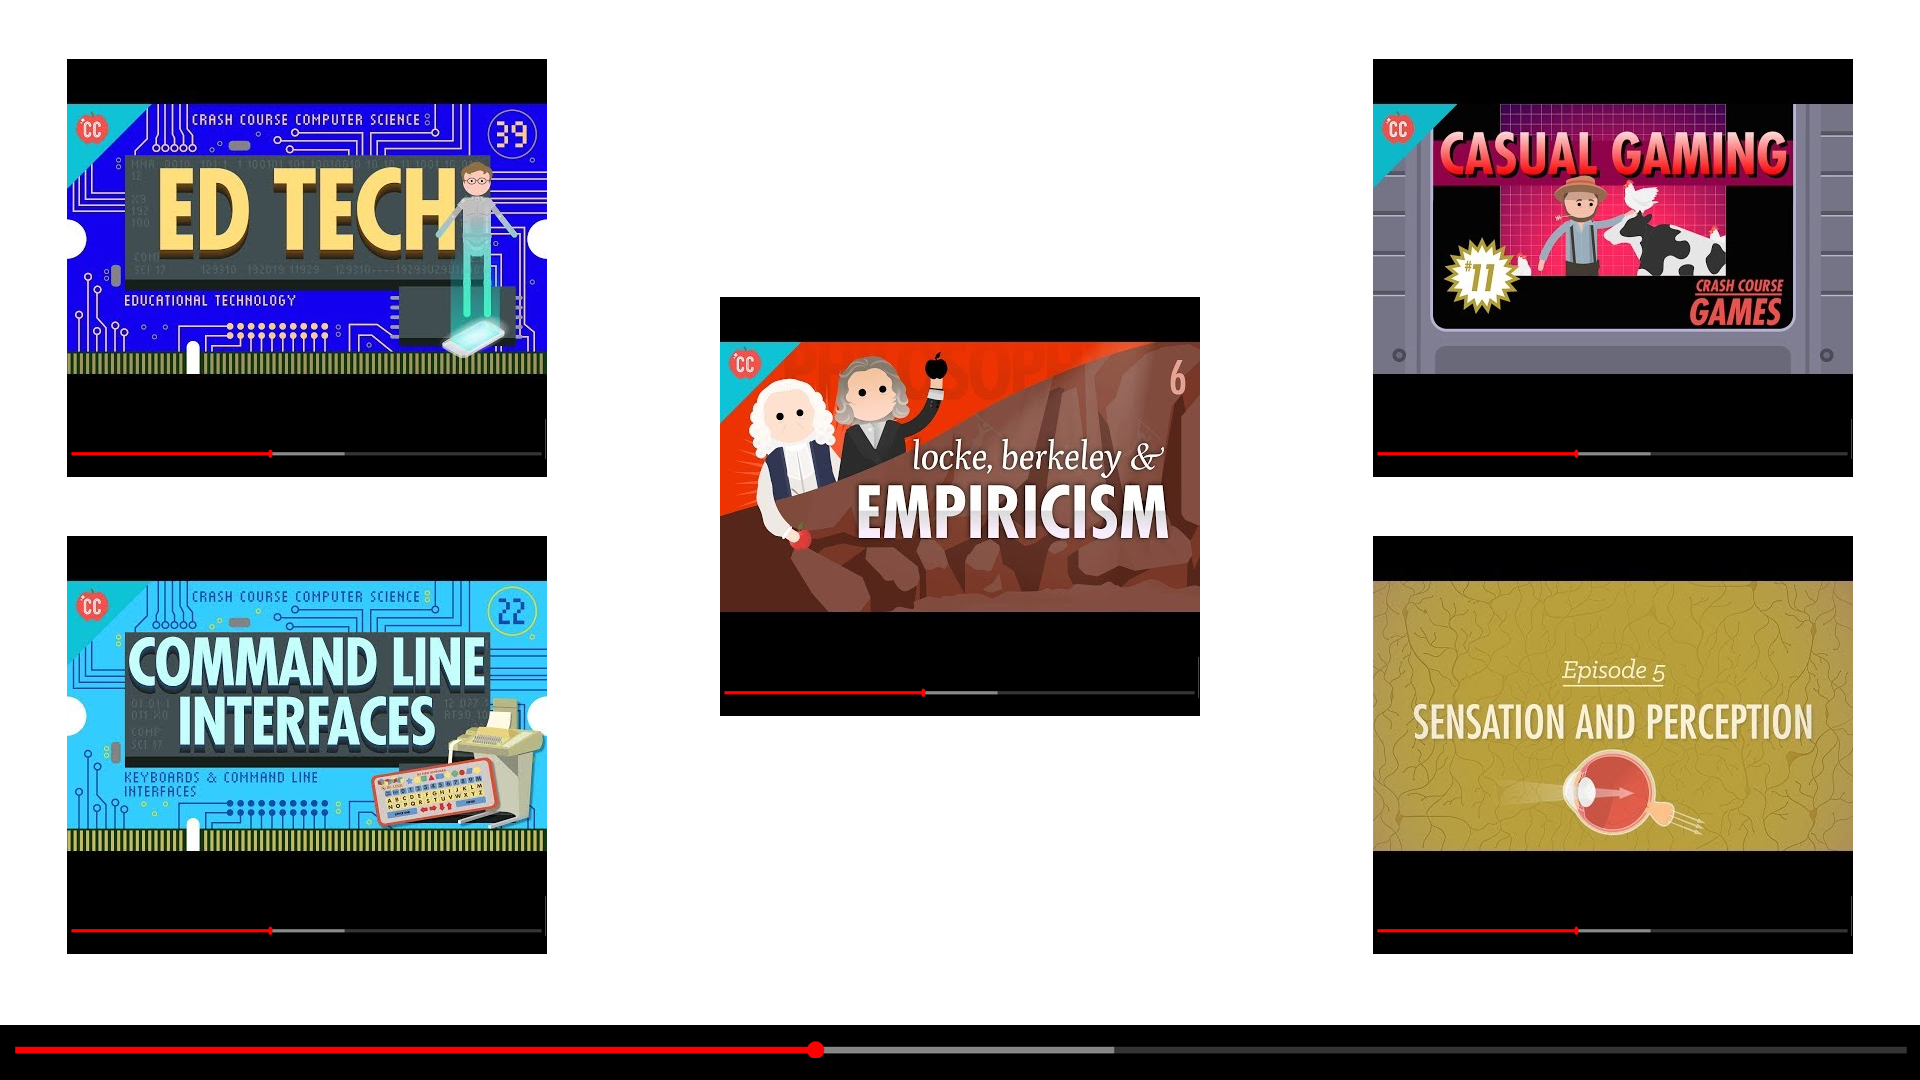
\includegraphics[width=1.35\textwidth, center]{images/global_scrub_bar_with_locals.png} % quotation marks make sure file name does not display
\caption{An example of how a global scrub bar looks like with local scrub bars. The global scrub bar manipulates the time of the local scrub bars but the local scrub bars can also be manipulated individually. Image credit: thumbnails from the educational show Crash Course (on YouTube).}
\label{images:global_scrub_bar_with_locals}
\end{figure}

% For now, let us focus on idea 2: how does one create a global time scrub bar in XIMPEL? The first straightforward solution (concept 2a) would be to have a global scrub bar mapped to individual scrub bars of each media type. This concept would marry idea 1 and 2 by having local time scrub bars and local time scrub bars.

%marrying local and global scrub bar
Moreover, idea 1 and 2 could be combined together by having a global scrub bar and local scrub bars (see figure \ref{images:global_scrub_bar_with_locals}). However, user studies would need to be done in order to validate the concept. Most web applications do not have multiple scrub bars, and therefore it might be a bit too overwhelming for the user.

% \begin{figure}
% \centering
% 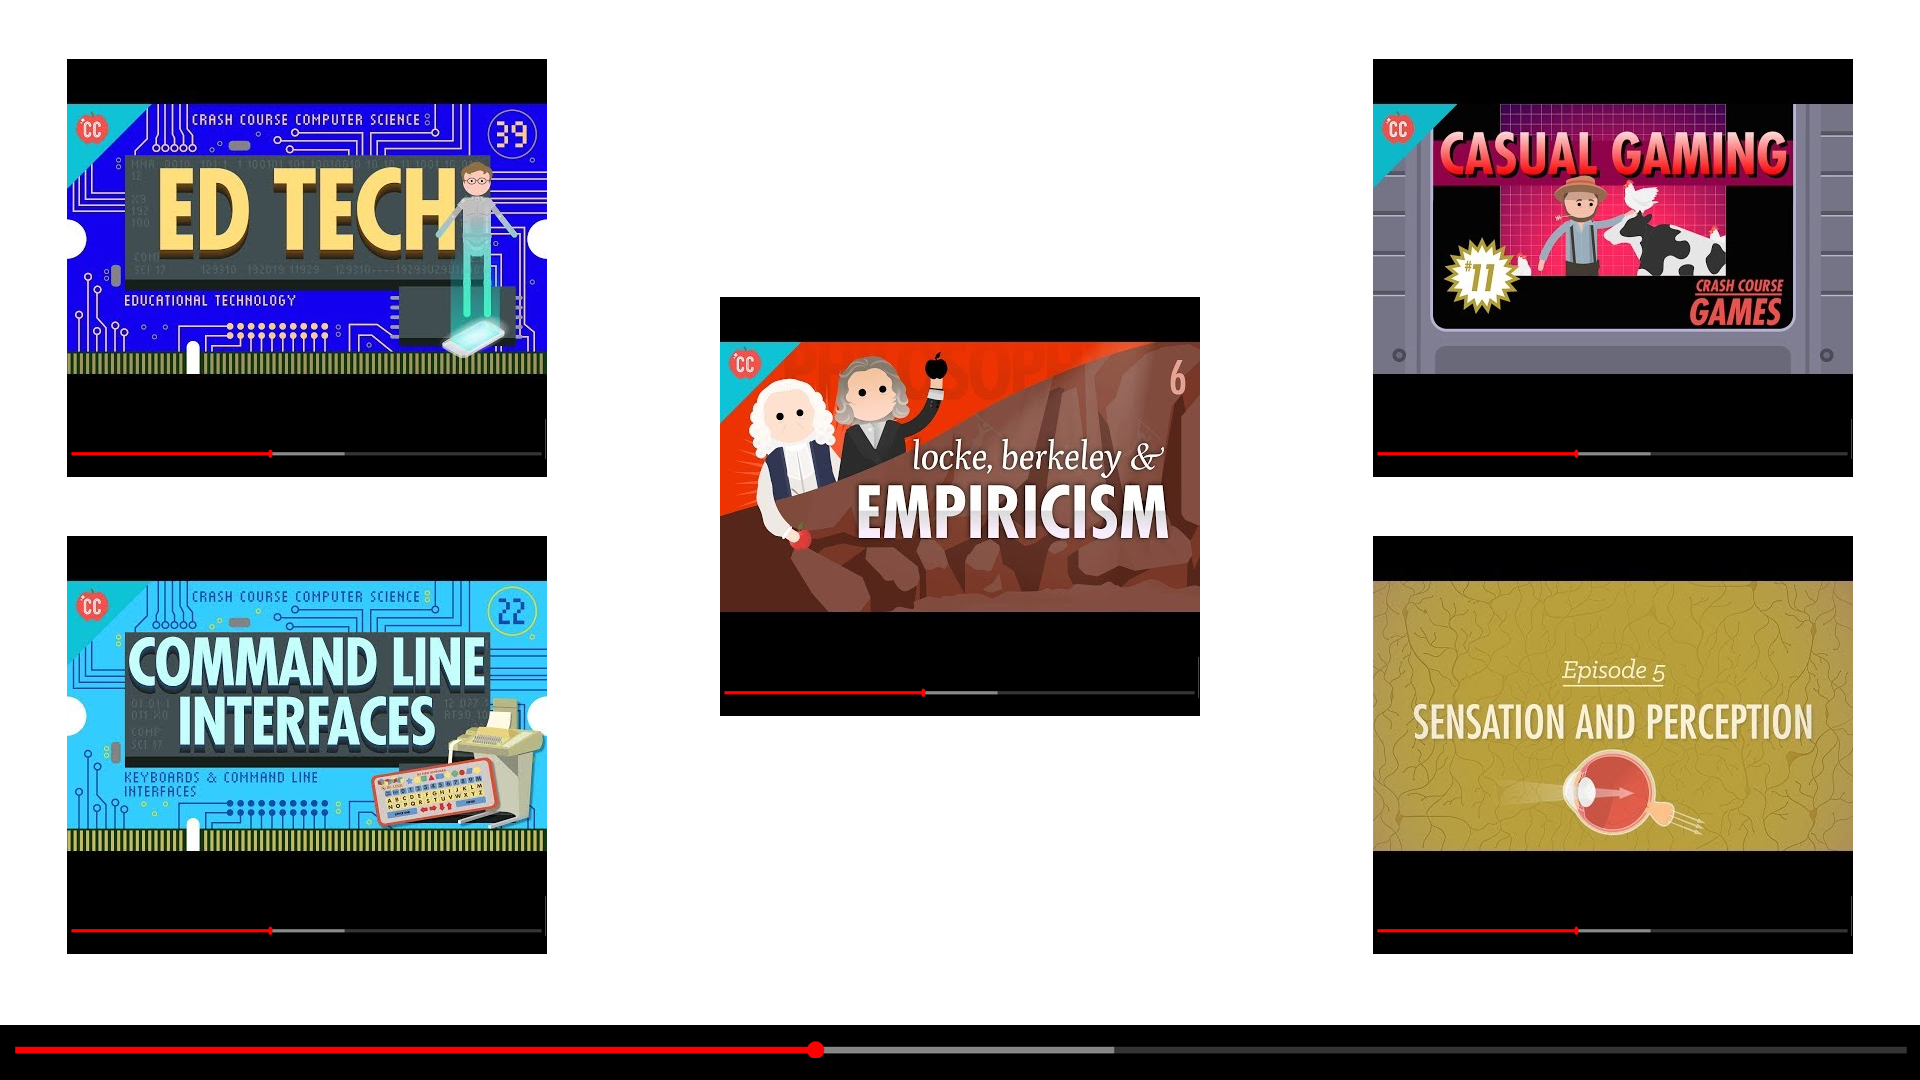
\includegraphics[width=1.35\textwidth, center]{images/global_scrub_bar_with_locals.png} % quotation marks make sure file name does not display
% \caption{An example of how a global scrub bar looks like with local scrub bars. The global scrub bar manipulates the time of the local scrub bars but the local scrub bars can also be manipulated individually. Image credit: thumbnails from the educational show Crash Course (on YouTube).}
% \label{images:global_scrub_bar_with_locals}
% \end{figure}


%talk about limitations of marrying ideas
The limitation of marrying these ideas is that when you time scrub the global one a design decision needs to be taken. If a user already scrubbed one time scrub bar locally and then scrubs globally, three different scrubbing situations could occur (see figure \ref{images:move_along_with_global}, \ref{images:move_along_with_offset} and \ref{images:catch_up}). Either the global time scrub bar resets the local time scrub bar to the original mapping where the global time scrub bar believes it to be. For example, a global time scrub bar is at 50\%, so all the local time scrub bars will be reset to 50\%. Another possibility is that local time scrub bars that have been meddled with, will move along according to the offset of the global time scrub bar. For example, the global time scrub bar is scrubbed from 30\% to 50\%, representing a 20\% increase. One local scrub bar has been scrubbed to 75\% prior. Then, it will increase to 95\% and the other local scrub bars, that have not been meddled with, will move to 50\%. The final possibility is that the meddled local scrub bars do not move if they are ahead of the global scrub bar, and will catch up and reset to the value of the global scrub bar when they are behind. Again figure \ref{images:move_along_with_global}, \ref{images:move_along_with_offset} and \ref{images:catch_up} visually clarify these difficulties.



% Three possibilities:
% 1. move along with scrub bar
% 2. move along with offset
% 3. catch up mechanic and otherwise do what you want

\begin{figure}
\centering
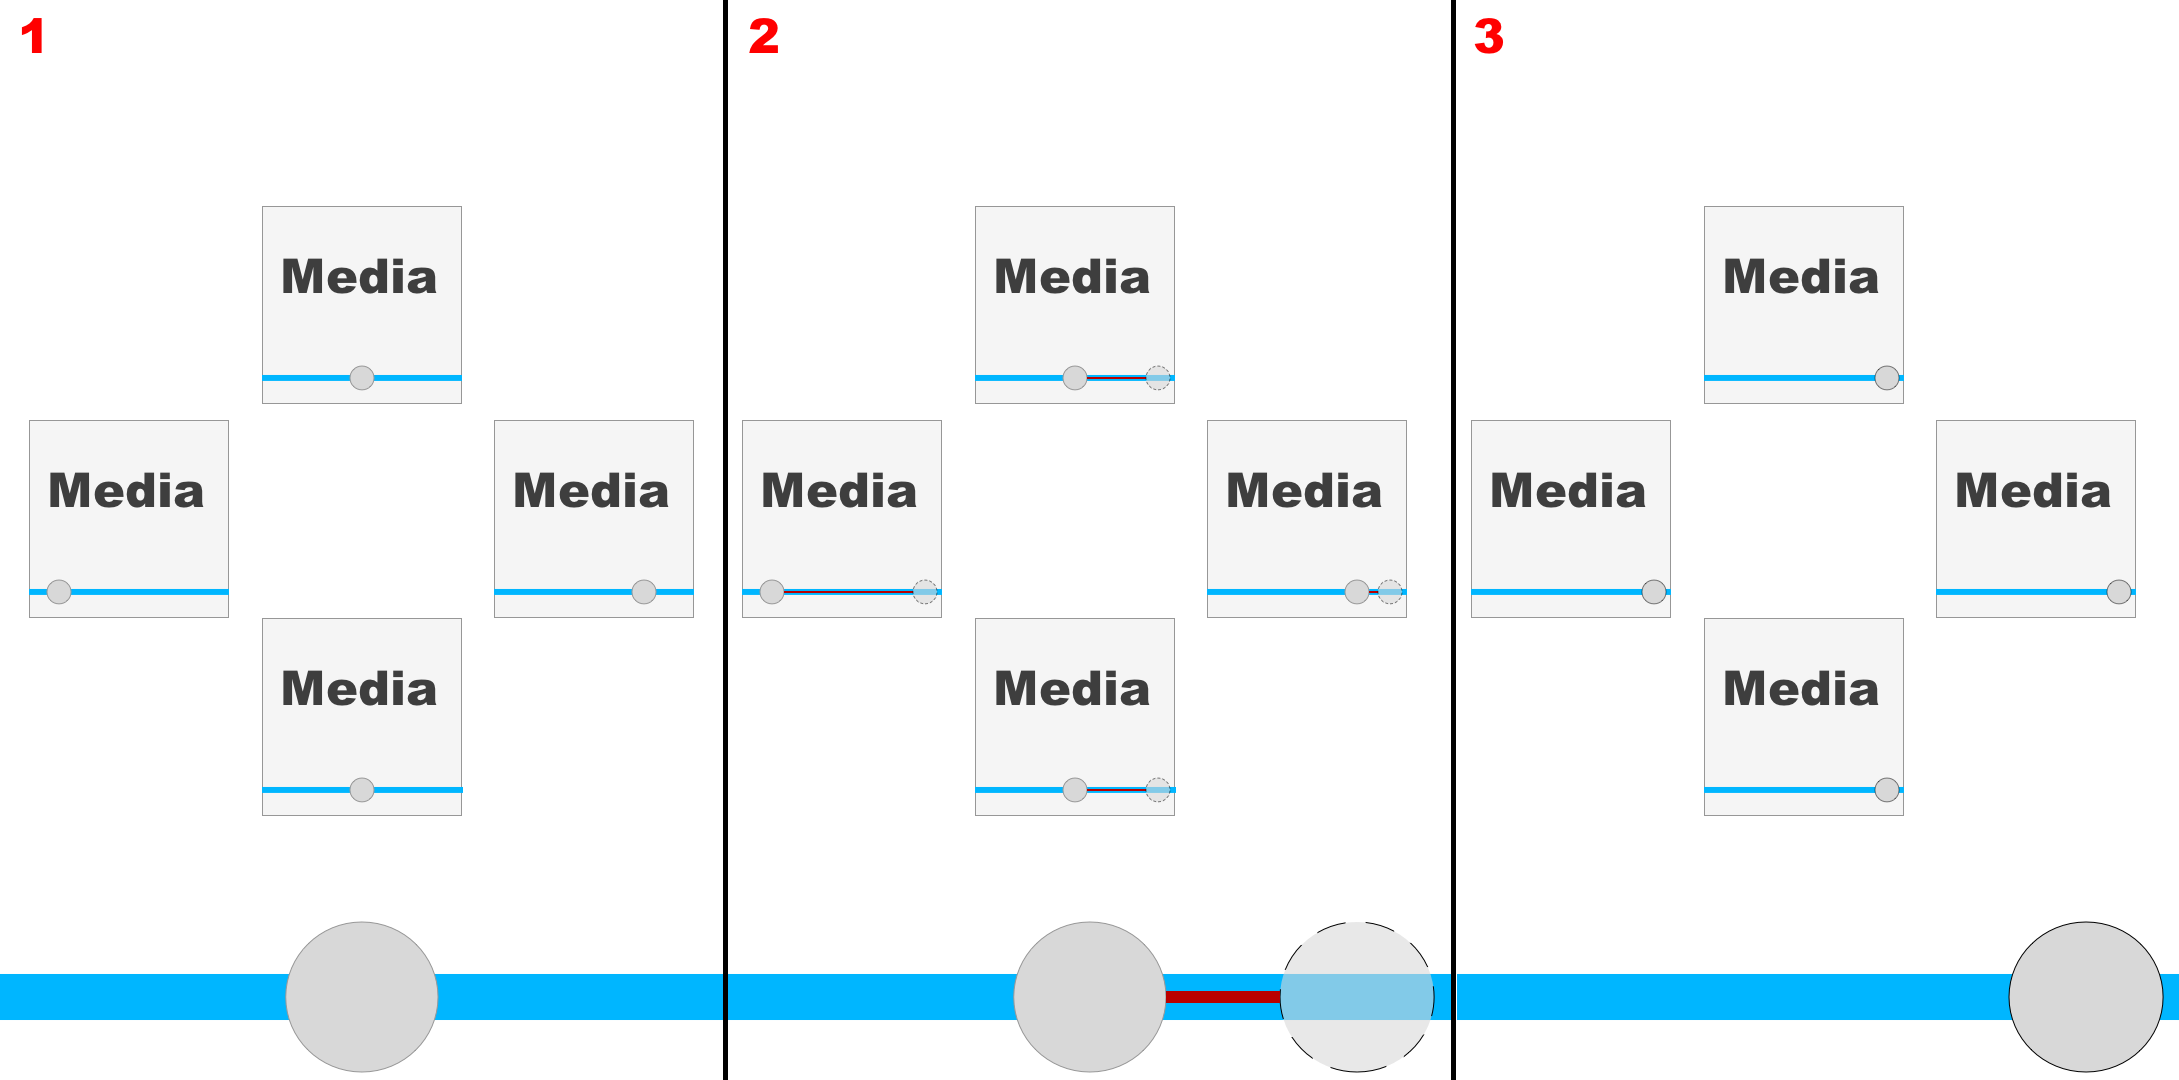
\includegraphics[width=1.35\textwidth, center]{images/move_along_with_global.png} % quotation marks make sure file name does not display
\caption{The global time scrub bar determines where all local scrub bars will resume playback.}
\label{images:move_along_with_global}
\end{figure}

\begin{figure}
\centering
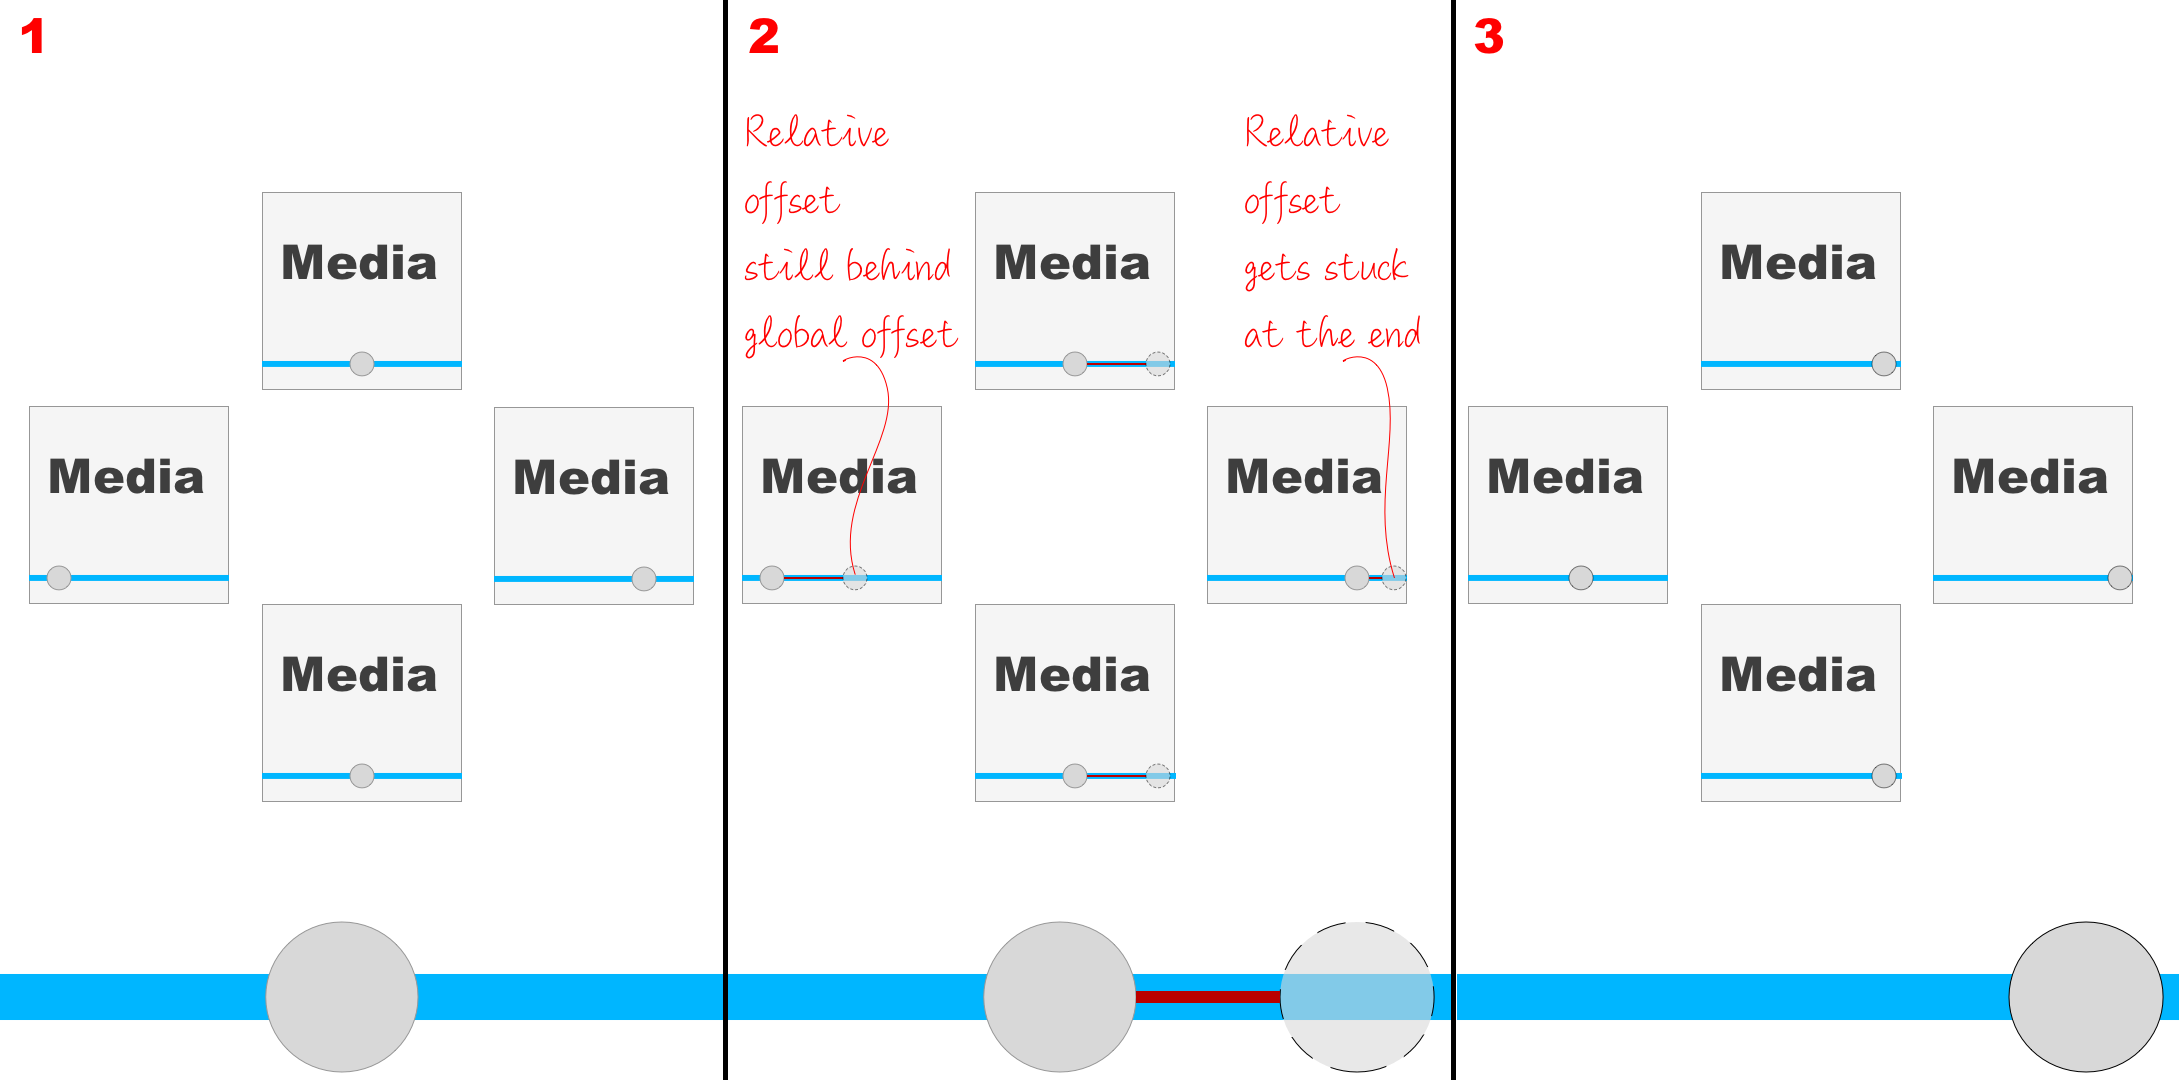
\includegraphics[width=1.35\textwidth, center]{images/move_along_with_offset.png} % quotation marks make sure file name does not display
\caption{The global time scrub bar determines the percentage offset that local scrub bars will give to their position in time.}
\label{images:move_along_with_offset}
\end{figure}

\begin{figure}
\centering
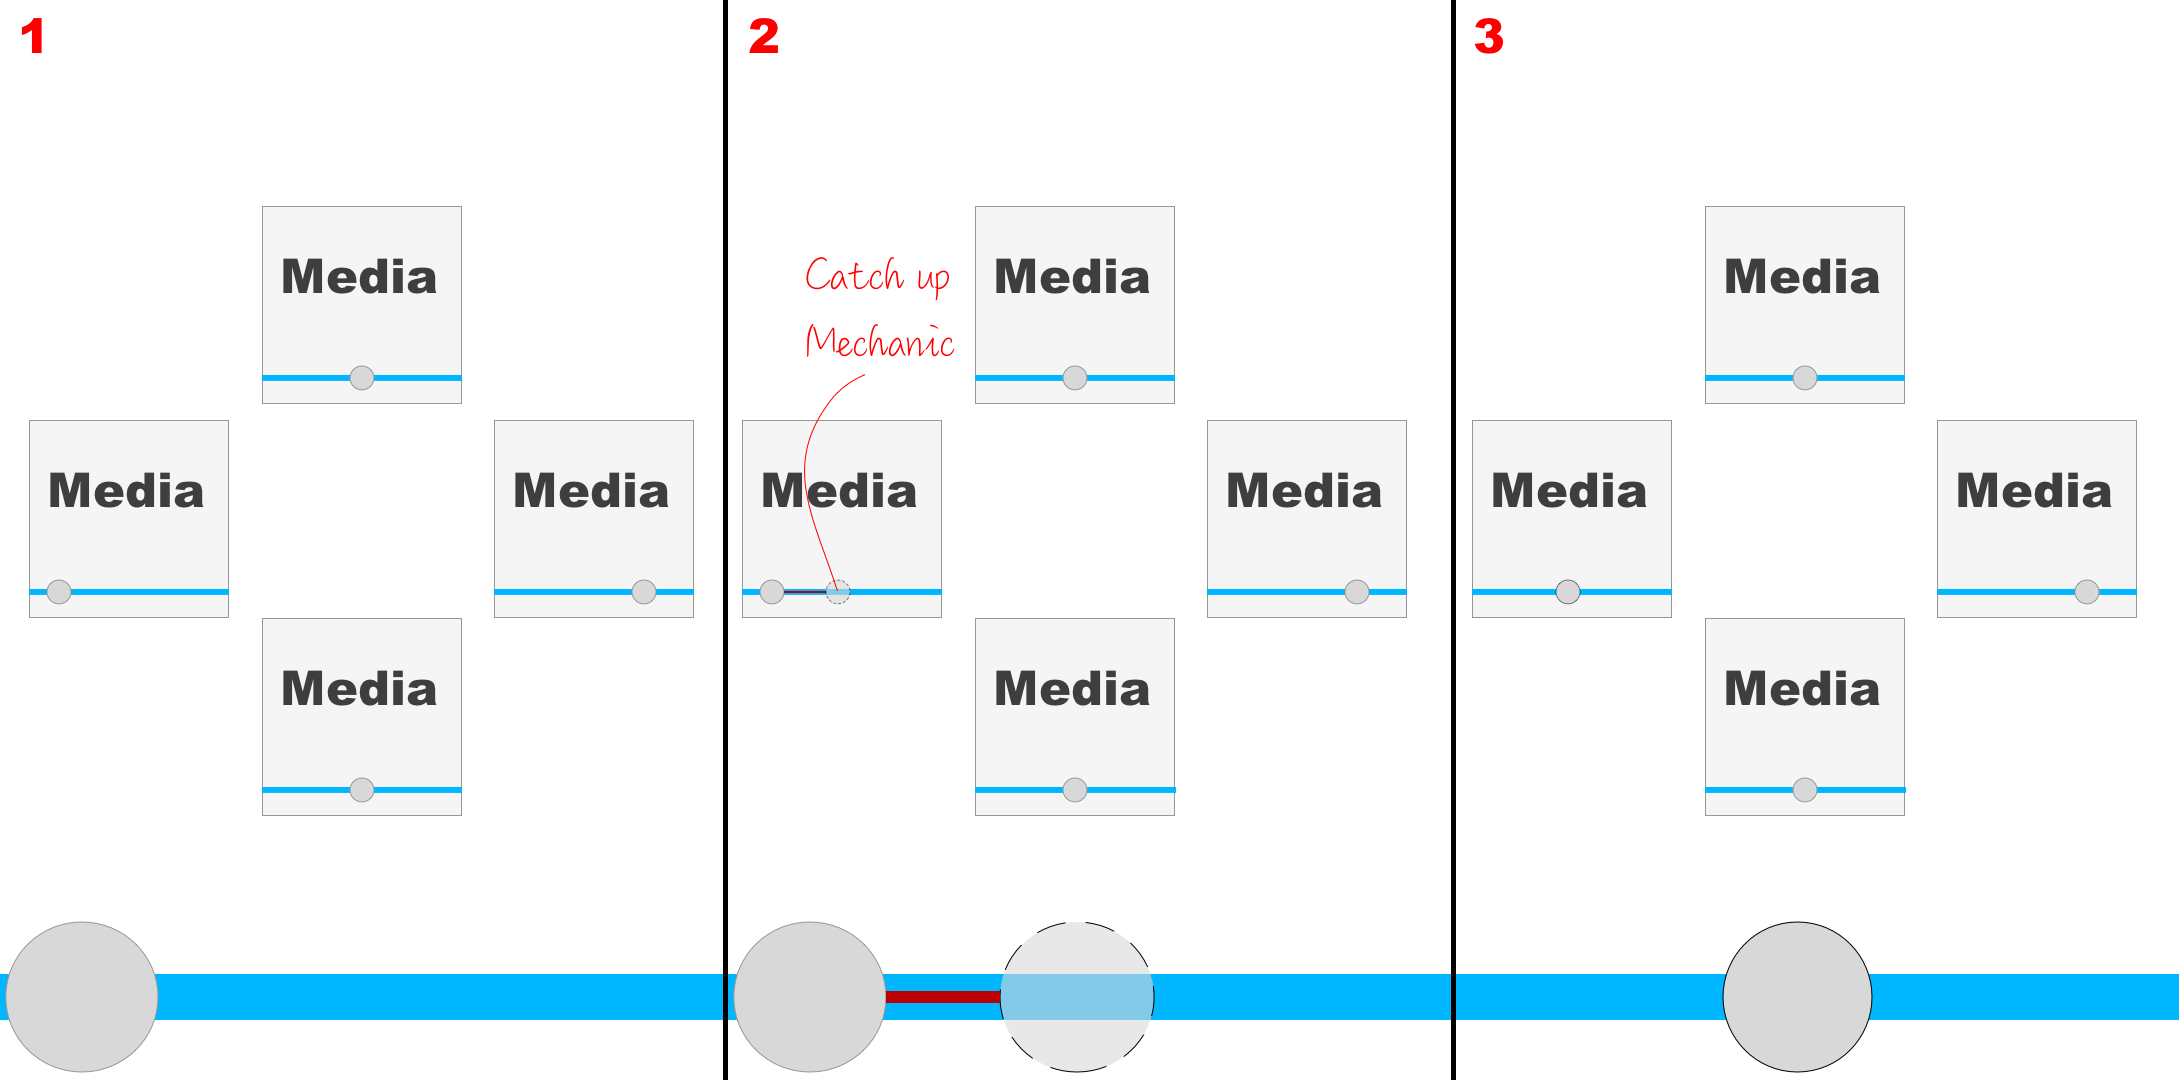
\includegraphics[width=1.35\textwidth, center]{images/catch_up.png} % quotation marks make sure file name does not display
\caption{The local scrub bars catch up with the global time scrub bar, but only if the local scrub bars are behind the global time scrub bar. There is also an inverse situation possible, here the local scrub bars will catch up to the global time scrub bar if they are ahead. This inverse situation is not shown in the figure. In the figure only one media item needs to catch up with its local scrub bar.}
\label{images:catch_up}
\end{figure}


\subsection{Time scrubbing: the difficulties introduced by users having choice}
The real difficulty is introduced not by the parallel player but by XIMPEL and the nature of interactive video and choice itself. One could ask herself or himself: if one scrubs from 30\% to 50\% but on the 40th percentile of the time line an overlay should be presented with a choice, should that choice be known to the user or not? The user may not know that there would be an overlay on the 40th percentile and therefore may not be aware of the choice. The user may also be specifically skipping to the 50th percentile, because the user knows there is an overlay there and wants to skip it.

In a single YouTube video this is less of an issue. YouTube overlays tend to be links to different videos that are less coherent compared to a certain group of hypermedia applications in XIMPEL. The user experience (UX) designers of YouTube presumably have decided that it is okay to skip these overlays. But should the user experience of XIMPEL be similar?

Both UX proposals would need to be tested. And while it is easy to copy the UX of YouTube, it is a less easy question to create a new UX in the case that overlays should be presented to a time scrubbing user. In order to answer this question I am forced to take inspiration from other systems or create something of my own and justify it.

Furthermore, is it desirable in XIMPEL presentations to inform the user that he or she is skipping overlays? Or is it more desirable to inform the user it is skipping a moment of choice. In the first scenario all overlays would need to be known by the user in advance. In the second scenario the user only needs to know whether there is any overlay present at certain moments in time, it does not matter how many overlays there are.

For this question, I take inspiration from the time scrubbing mechanism that professor David J. Malan and his colleagues have developed for the course CS50 at Harvard. The reason for that is because it solves a similar problem and it was usable for me when I took the course years ago. The problem that they solved is that during a lecture a student would be introduced to multiple topics or sub-topics. Since the level difference between the students is quite big, some students may want to skip certain topic. By creating a time scrub bar that allows students to knowingly skip a certain lecture topic, they give the power (the choice) to students to do so. In other words, their problem is also a problem about choice, albeit a different form of choice. 

% TO DO: You left at the CS50 interface.

Figure \ref{images:cs50_player} will show the user interface design. Like CS50 we highlight certain points of the time scrub bar. By doing this, the user is able to know when there will be a potential choice. When the user hovers over such a point, the user will see all possible choices that he or she can make at such a point. This interface is relevant for people who already went through a XIMPEL presentation. In some cases, the XIMPEL author may want to disable this feature since not knowing when certain decisions ought to be made potentially add value to the UX of a XIMPEL application.

This interface works well for one media item? Would such an interface scale for multiple media items? For that dear reader I ask you to use your imagination. Imagine multiple media items, for example, two videos, one audio and one image somewhere on the screen. Got it? Amazing! When all media items have their own time scrub bar -- or in the case of the image at least a time line which you cannot interact with -- then highlighting certain points on the time scrub bar or time line is not an issue. In this way it does scale. However, it is also possible to put all the highlighted points at a global time scrub bar. The possible disadvantaged is that a user cannot identify to which media item the choice belongs to, which is a piece of information that may or may not be important depending on the XIMPEL presentation being played.

\begin{figure}
\centering
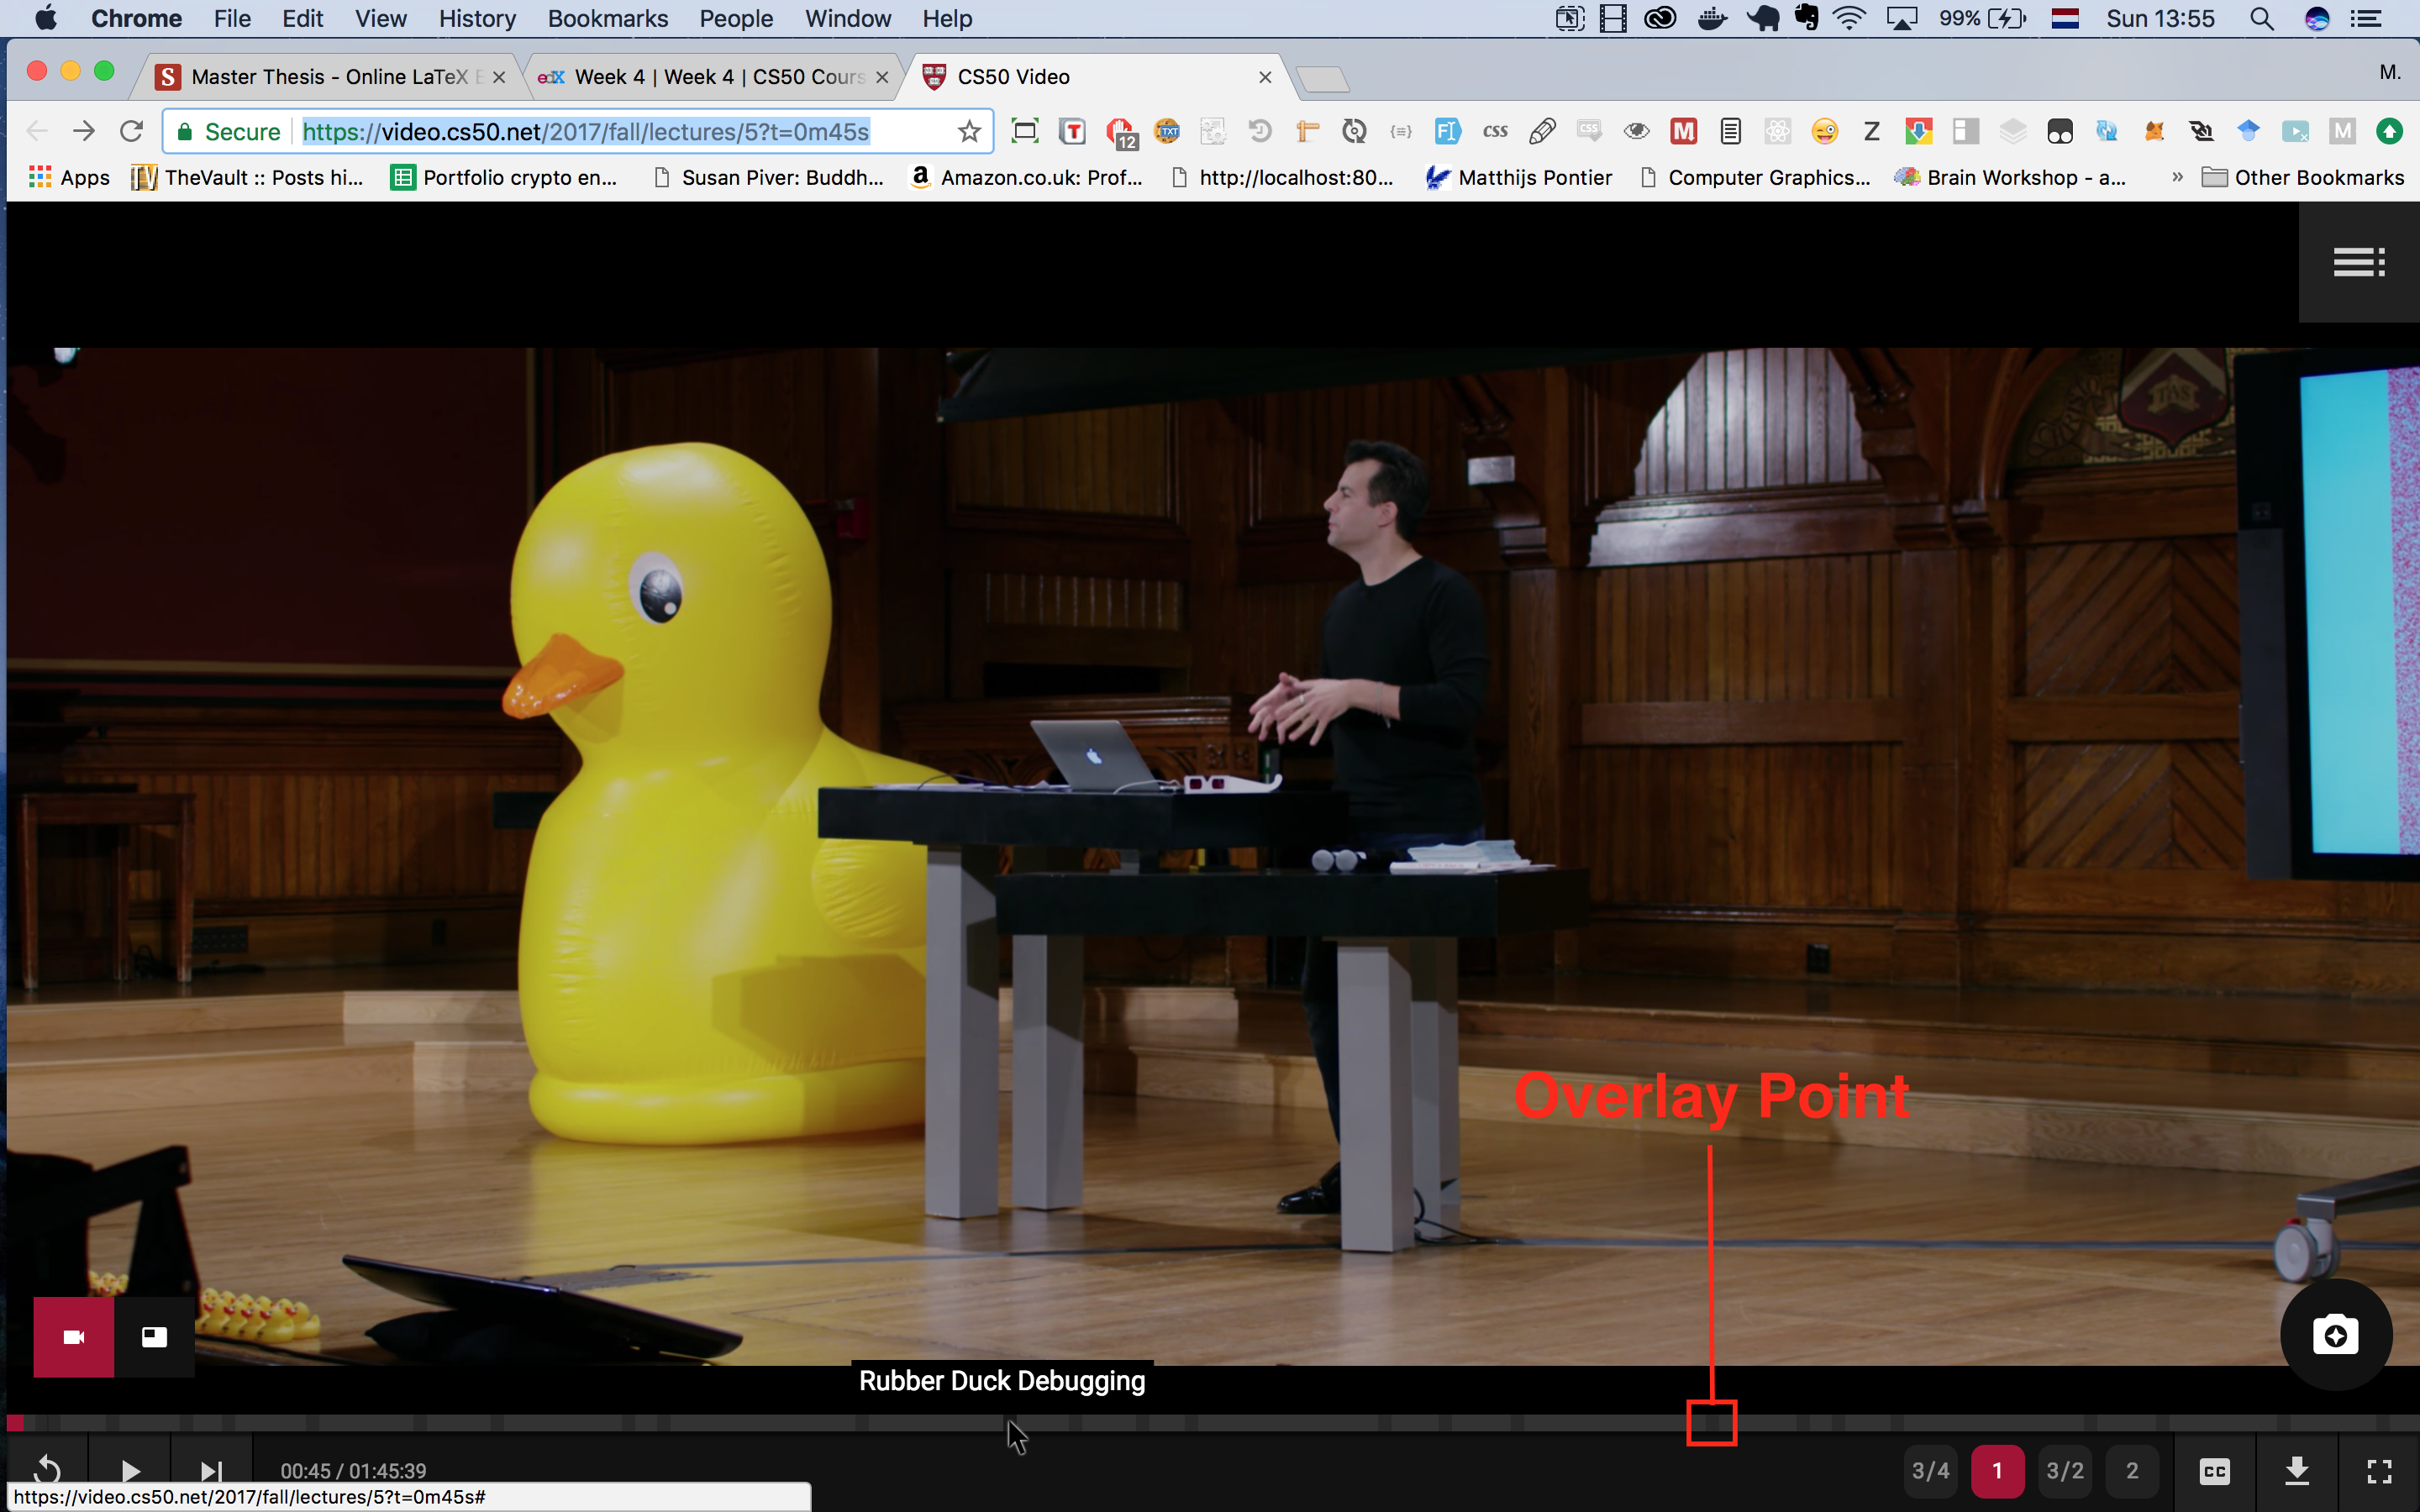
\includegraphics[width=1.35\textwidth, center]{images/cs50_player.png} % quotation marks make sure file name does not display
\caption{An example of the CS50 player. In this screenshot the mouse hovered over an overlay point called Rubber Duck Debugging.}
\label{images:cs50_player}
\end{figure}

\section{Between subject time scrubbing in XIMPEL}
Now that I have outlined which possible design dilemma's by having choice within XIMPEL and the newly built parallel player introduces within a subject, let us look what interactive video or rather XIMPEL itself introduces. What if we do not want to time scrub within a subject but between subjects? From a user experience point of view this is entirely possible because users may experience the interactive video as a whole, and perhaps they would want to skip certain scenes, or maybe skip halfway.

It is important to understand that this is a wicked problem, meaning: ``a problem with multiple plausible solutions as well as multiple subjective interpretations of such solutions. \cite{olsson2014}'' The paper of Carl Magnus Olsson, Staffan Björk and Steve Dahlskog goes into detail about what wicked problems are, how it relates to design (and game-design in particular) and how to deal with them \cite{olsson2014}. For now, it suffices to understand what a wicked problem is, in our case devizing solutions really means making compromises between ease of use and having more information. I will present two different designs which emphasizes one or the other. In order to see which design would be better, user studies would need to be conducted for which I unfortunately lack the time.

% 1: show full graph
We could show more information by having a screen that displays the full interaction graph of XIMPEL. The user would be able to see at exactly which point a choice would be made and would be able to scrub along the time graph (it is not a time line anymore) and land at the point where he or she wants to be. The issue with this is that this may, in some cases, neglect the idea of interactive video. By giving a user the possibility of seeing the interaction points, the author of a XIMPEL application would be forced to give away a part of the surprise. An example of such a graph is shown in figure \ref{tikz:full_graph}.

% For scaling see: https://tex.stackexchange.com/questions/4338/correctly-scaling-a-tikzpicture
% For captioning it see: https://tex.stackexchange.com/questions/28258/what-is-the-correct-way-to-caption-a-tikzpicture
% The picture: is tested at: https://www.sharelatex.com/project/5ab8f520af30be4134f56286
\begin{figure}
\centering
\scalebox{0.5}{
\begin{tikzpicture} %[scale=0.5]
\begin{scope}[every node/.style={circle,thick,draw, align=center}]

    %Subject: De Bonte Hen 
    \node (MenuDeBonteHen) at (0,0) {Menu\\De Bonte Hen};
    \node (WalkToHetJongeSchaap) at (5,5) {Walk to\\Het Jonge Schaap};
    
    \node (QuizBonteHenIntro) at (5,0) {Quiz\\De Bonte Hen intro};
    \node (QuizMenuDeBonteHen) at (10,0) {Quiz Menu\\De Bonte Hen};
    \node (WrongBonteHenQuiz) at (15,5) {Wrong answer};
    \node (CorrectBonteHenQuiz) at (15,-5) {Right answer};
    \node (CorrectBonteHenQuizInfo) at (20,-5) {Correct answer information};
    
    \node (TourOfMolenDeBonteHen) at (5,-5) {Tour of windmill\\De Bonte Hen};
    
    %Subject: Het Jonge Schaap 
    \node (MenuMolenHetJongeSchaap) at (10,15) {Menu\\Molen Het Jonge Schaap};
    \node (MenuDeZoeker) at (15,21) {Menu\\De Zoeker};
    
    \node (QuizJongeSchaapIntro) at (15,15) {Quiz\\Het Jonge Schaap};
    \node (QuizJongeSchaapMenu) at (20,15) {Quiz\\Het Jonge Schaap};
    \node (WrongJongeSchaapQuiz) at (25,20) {Wrong answer};
    \node (CorrectJongeSchaapQuiz) at (25,10) {Right answer};
    \node (CorrectAnswerJongeSchaapInfo) at (30,10) {Correct answer information};
    
    \node (TourOfMolenHetJongeSchaap) at (15,10) {Tour of\\Molen Het Jonge Schaap};
    
    %Subject: De Zoeker
    \node (DeZoeker) at (20,21) {De Zoeker\\(subtree truncated)};
    
\end{scope}

\begin{scope}[>={Stealth[black]},
            %   every node/.style={fill=white,circle},
              every edge/.style={draw=red,very thick}]
              
    %Subject: De Bonte Hen
    \path [->] (MenuDeBonteHen) edge node {} (WalkToHetJongeSchaap);
    \path [->] (MenuDeBonteHen) edge node {} (QuizBonteHenIntro);
    \path [->] (MenuDeBonteHen) edge[bend left=5] node {} (TourOfMolenDeBonteHen);
    
    \path [->] (TourOfMolenDeBonteHen) edge[bend left=5] node {} (MenuDeBonteHen);
    
    \path [->] (QuizBonteHenIntro) edge node {} (QuizMenuDeBonteHen);
    \path [->] (QuizMenuDeBonteHen) edge node {} (WrongBonteHenQuiz);
    \path [->] (WrongBonteHenQuiz) edge[bend right=10] node {} (MenuDeBonteHen);
    \path [->] (QuizMenuDeBonteHen) edge node {} (CorrectBonteHenQuiz);
    \path [->] (CorrectBonteHenQuiz) edge node {} (CorrectBonteHenQuizInfo);
    \path [->] (CorrectBonteHenQuizInfo) edge[bend left=60] node {} (MenuDeBonteHen);
    
    %Subject: Het Jonge Schaap
    \path [->] (WalkToHetJongeSchaap) edge node {} (MenuMolenHetJongeSchaap); %Transition
    
    \path [->] (MenuMolenHetJongeSchaap) edge node {} (MenuDeZoeker);
    \path [->] (MenuMolenHetJongeSchaap) edge node {} (QuizJongeSchaapIntro);
    \path [->] (MenuMolenHetJongeSchaap) edge[bend left=5] node {} (TourOfMolenHetJongeSchaap);
    
    \path [->] (TourOfMolenHetJongeSchaap) edge[bend left=5] node {} (MenuMolenHetJongeSchaap);
    
    \path [->] (QuizJongeSchaapIntro) edge node {} (QuizJongeSchaapMenu);
    \path [->] (QuizJongeSchaapMenu) edge node {} (WrongJongeSchaapQuiz);
    \path [->] (WrongJongeSchaapQuiz) edge[bend right=5] node {} (MenuMolenHetJongeSchaap);
    \path [->] (QuizJongeSchaapMenu) edge node {} (CorrectJongeSchaapQuiz);
    \path [->] (CorrectJongeSchaapQuiz) edge node {} (CorrectAnswerJongeSchaapInfo);
    \path [->] (CorrectAnswerJongeSchaapInfo) edge[bend left=65] node {} (MenuMolenHetJongeSchaap);
    
    %Subject: De zoeker
    \path [->] (MenuDeZoeker) edge node {} (DeZoeker);
    
\end{scope}
\end{tikzpicture}
}
\caption{In this figure a part of full interaction graph of the XIMPEL presentation of the Zaanse Schaans is shown. Users who would like to scrub between subject could see a graph like this, and click on any part of the edge to indicate how far they want to start in a subject. A graph like this could be shown in the upper right corner by clicking on a button, for example. What is not shown in this image is that overlays could be displayed on any part of the edge as well for additional scrubbing information.}
\label{tikz:full_graph}
\end{figure}


In normal time scrubbing this is not a problem. Consider a horror movie -- where there are a lot of surprises. When a person scrubs further along the time line, he or she has no idea what to expect. This is because nothing is highlighted other than the time. With showing the full interaction graph it may not only be needed to show where the interaction points are, but also which interaction points. Whether users prefer a full interaction graph with only nodes and edges going out of nodes or also see labeled possible interactions on the nodes would require user testing. 

% 2: show a simple way to skip scenes with overlays as is possible within current XIMPEL
The simpler way of doing time scrubbing in XIMPEL is creating a scene skipping feature. With the current capabilities of XIMPEL this is already possible. It is even possible to show all possible options for the next scene as an overlay that the user could click or tap on. While it is a crude way of time scrubbing, it is an easier interface and perhaps therefore more usable. An example of this is done in the Zaanse Schans XIMPEL presentation (see \url{http://classic.ximpelapps.nl/zaanseschans_html5}).

\section{Interaction of within and between subject time scrubbing}
% D. 50% of 5th subject --> leave state in a certain way --> what if user scrubs bag to it?
When a user scrubs within a subject, as soon as the user moves to scrub time between subjects it begs the question whether a XIMPEL application should remember the scrubbed state within the subject or whether it should not. If it should, then the concept of time becomes slightly different. For example, a user scrubs the 50th percentile of the fifth subject with the between subject scrubber, then if the user left the state of that subject in a certain way it needs to be recalculated what it means to scrub to the 50th percentile of it with respect to the offset of where the user left it. Imagine a user clicking on the middle of the upper arrow between \textit{Menu De Bonte Hen} and \textit{Tour of windmill De Bonte Hen} in figure \ref{tikz:full_graph} (lets call this user action A). Then the user would be transported to the middle of the video that is associated to \textit{Menu De Bonte Hen}. If the user, then suddenly clicks somewhere completely differently on an edge in the time graph (user action B), and then performs user action A again after a couple of second -- perhaps of boredom. Should a XIMPEL presentation remember that it already was playing from the 50th percentile, and therefore conclude that since the user clicked on the middle of the edge again replay the 50th percentile or add it as an offset? It depends on the intent of the author with their XIMPEL presentation, but both are options.

% E. 50% of 5th subject --> leave state within a certain way (but is forgotten) --> user scrubs back to it in the same way and sees the same thing
% F. User *first* needs to scrub between subject and is only then able to scrub within subject.
There are two other possibilities that make the interaction for between subject time scrubbing and within subject time scrubbing easier. The first possibility is alluded to in the previous paragraph, which is not to remember the within subject state. For example, when a user scrubs to the 50th percentile of the fifth subject, then a user would see the fifth subject playing at the 50th percentile point in time, which is always the same, namely: the 50th percentile point in time of the fifth subject. A second option could be to not intermix between subject time scrubbing and within subject time scrubbing, but having two layers. In this design a user would first need to choose to which subject they want to travel to and when that subject loads, only then is it possible to time scrub within that subject. The latter option is easier to implement since separated conceptual concerns translates to compartmentalized code (e.g. different classes and different files). One could imagine figure \ref{tikz:full_graph} still being shown in the upper right corner when a button is clicked. When the user clicks on a node, then the subject is loaded and only then is it possible to scrub within the subject using time line sliders as seen earlier in the section \textit{Time scrubbing: the difficulties introduced by the parallel player}.

\section{Conclusion}
% Summarizing
Implementing time scrubbing within hypermedia frameworks stumbles upon a lot of questions and little answers. This topic has not been explicitly studied and because of that this chapter has been written. Specifically three areas with design related questions have been identified:
\begin{itemize}
    \item Within subject time scrubbing.
    \item Between subject time scrubbing.
    \item The interaction of within subject time scrubbing and between subject time scrubbing.
\end{itemize}

Another design topic written about -- albeit in a less structured way -- has to do with the overlay in XIMPEL. Does the possibility of choice need to show up in a time scrub bar? If no, then we are done. If yes, then there are three areas to consider:
\begin{itemize}
    \item Presenting possible future overlays within a single media item (related to within subject time scrubbing).
    \item Presenting possible future overlays within multiple media items and different media types (related to within subject time scrubbing).
    \item Presenting possible future overlays while time scrubbing between subjects (related to between subject time scrubbing).
\end{itemize}

% Integrating research
Possible designs have been proposed and have been inspired from previous research. Presenting possible overlays in the future could be implemented in a similar way the video player of CS50 or \cite{automaticsection2015} do. Except instead of showcasing summarized labels of what the video is about at that current point in time, the labels will be about what overlays they are and what for effect they may have on the user. Inspiration for within subject time scrubbing mostly came from the study that multiple time lines in order to fine-tune time scrubbing \cite{multipletimeline1999}. Knowing that it sometimes is useful to have multiple time scrub bars gave rise to the idea to split time scrubbing up into a global time scrub bar and local scrub bars (one per media item). The design approaches for between subject scrubbing have been inspired by the research of \cite{videotree2010}. Abstracting subjects away as a node and conceiving that it could be possible to time scrub a whole graph has been sparked by the idea that it is possible to manipulate time through multiple trees, such as the ones presented in \cite{videotree2010}. 

% Limitations of this analysis
A limitation of this exploration is that this means that a lot of research did not directly go into the design of time-scrubbing within XIMPEL. The biggest example is manipulating objects within a video \cite{nguyen2013, shah2013, goldman2008, dragicevic2008, kimber2007}. Another example is research done on time-scrubbing systems within the context of MOOCs. Ideas of user statistics\cite{kim2014}, word clouds\cite{yadav2015} did not make it. What did make it was showing points of interests through overlays\cite{yadav2015}. 

Another glaring limitation is that there is the implicit assumption that all media items have the same time! This limitation has been found out too late in order to change the analysis, and it would make matters most likely even more complicated. It would be odd to have a global time scrub bar track everything in a relative fashion if one media item only takes 5 seconds of playback and another media item 500 seconds of playback. The full length of the global time scrub bar has to be pegged to the longest playing media item perhaps, but the implications of doing so would not be clear, especially not if some media items have infinite time.

% Where to go from now
Future work could be done on doing user studies or by choosing a subset of all the possible designs outlined in this chapter and directly implementing it. In the first case, user studies would need to indicate to what extent users want to be able to have time scrubbing abilities. And high-fidelity mockups are possible by using XIMPEL and local scrubbing. A target group of interest to test these mockups with would be people who like to go to museums, since XIMPEL as a framework seems to be rising in popularity. Another one would be students since they seem to be one of the most tech-savvy mainstream general groups, and they are relatively easy to recruit. 

Regarding implementation, the idea of what a media item is changes. Not only is a media item able to track time but it is also able to scrub time. Moreover, in some design ideas this information needs to be passed something controlling the subject and when it changes to another. So the XIMPEL player in XIMPEL JS or the `Subject` component in XIMPEL React need time-tracking and time-scrubbing capabilities. These code entities need information from the media items, since it needs to know what their internal playback position is.

One design and implementation approach is to stay close to the XIMPEL design philosophy, which is to keep things simple and not to overthink it. At first I thought this meant: there is a global time scrub bar which determine the time scrub bars of media items (this is exactly \ref{fig:normal_time_scrubbing}), no possible future overlays are shown at the time scrub bar and overlays could already be used to skip individual scenes. However, because of the limitation regarding the global time scrub bar a more pragmatic approach is to only allow for local time scrub bars. This has been programmed into XIMPEL JS and XIMPEL React as the attribute `timescrubbing="true"` (the default is false).

Another form of future work would be to do a conceptual analysis on a partial global time scrub bar. This would be a global time scrub bar that is linked to media items that a XIMPEL author believes it should be linked with, and the unlinked media items have a local scrub bar (not connected to the global one) or none at all. Showcasing the implications of this may yield to fruitful research efforts regarding time scrubbing and hypermedia.

So, what needs the ability to go foreward and backward in time? A media item? A subject? A whole graph? These are the three levels that have been discussed in this exploration. Despite that, there are many stones left unturned and many corners regarding this research area uncovered. Indeed, it might be clear: in this problem there is no rest for the wicked.